\documentclass{report}
% Change "article" to "report" to get rid of page number on title page
\usepackage{amsmath,amsfonts,amsthm,amssymb}
\usepackage{setspace}
\usepackage{Tabbing}
\usepackage{fancyhdr}
\usepackage{lastpage}
\usepackage{extramarks}
\usepackage{chngpage}
\usepackage{soul,color}
\usepackage{listings}
\usepackage{enumerate}
\usepackage{graphicx,float,wrapfig}
\usepackage{pifont}
\usepackage{graphicx}
\usepackage[english]{babel}
\usepackage{tikz}
\usepackage[]{algorithm2e}
% In case you need to adjust margins:
\topmargin=-0.45in      %
\evensidemargin=0in     %
\oddsidemargin=0in      %
\textwidth=6.5in        %
\textheight=9.0in       %
\headsep=0.25in         %

\title{Assignment 2 - Comp 632 - Machine Learning}

% Homework Specific Information
\newcommand{\hmwkTitle}{Assignment 2}                     % Adjust this
\newcommand{\hmwkDueDate}{Wednesday, February 18 2015}                           % Adjust this
\newcommand{\hmwkClass}{COMP 632}


\newcommand{\hmwkClassInstructor}{Dr. Doina Precup}
\newcommand{\hmwkAuthorName}{Geoffrey Stanley}
\newcommand{\hmwkAuthorNumber}{260645907}
\newcommand{\Pp}{\mathbb{P}}
\newcommand{\Ev}{\mathbb{E}}
\newcommand{\cov}{\text{Cov}}
\newcommand{\Z}{\mathbb{Z}}
\newcommand{\R}{\mathbb{R}}
\newcommand{\dd}{\, \mathrm{d}}

% Setup the header and footer
\pagestyle{fancy}                                                       %
\lhead{\hmwkAuthorName}                              %
\chead{}
\rhead{\hmwkClass: \hmwkTitle}                                          %

\lfoot{}
\cfoot{}                                                                %
\rfoot{Page\ \thepage\ of\ \pageref{LastPage}}                          %
\renewcommand\headrulewidth{0.4pt}                                      %
\renewcommand\footrulewidth{0.4pt}                                      %

% This is used to trace down (pin point) problems
% in latexing a document:
%\tracingall
\definecolor{mygreen}{rgb}{0,0.6,0}
\lstset{commentstyle=\color{mygreen}, frame=single,  language=R, showspaces=false, showstringspaces=false}

%%%%%%%%%%%%%%%%%%%%%%%%%%%%%%%%%%%%%%%%%%%%%%%%%%%%%%%%%%%%%
% Make title
\title{\vspace{2in}\textmd{\textbf{\hmwkClass:\ \hmwkTitle}}\\
\normalsize\vspace{0.1in}\small{Due\ on\ \hmwkDueDate}\\
\vspace{0.1in}\large{\textit{Presented to \hmwkClassInstructor}}\vspace{3in}}
\date{}
\author{\textbf{\hmwkAuthorName}\\
    \textbf{Student ID: \hmwkAuthorNumber}}
%%%%%%%%%%%%%%%%%%%%%%%%%%%%%%%%%%%%%%%%%%%%%%%%%%%%%%%%%%%%%

\begin{document}
\maketitle
\section*{Question 1}
\subsection*{A)}
For a function to be considered a kernel function the kernel matrix defined as
$K_{ij}=K(x_i,x_j)$ must have two properties:
\begin{enumerate}
  \item be symmetric
  \item be positive semidefinite
\end{enumerate}
As such, a Kernel matrix must abide by the following:
\begin{equation}
  K_{ij} = K_{ji}
\end{equation}
\begin{equation}
  z^{T}Kz\geq 0
\end{equation}
Where $z$ is an arbitrary vector. \\

A kernel function is also one that can be expressed as a dot product of the feature
vectors of the instances:
\begin{equation}
  K(x,z) = \phi (x) \cdot \phi (x)
\end{equation}
where $\phi$ is a feature maping of input features to a vector space. Further more,
as described by Bishop(2006) p.296 a kernel function can be a construction of kernel
functions such that
\begin{equation}
  k(x,z) = k_1(x,z) + k_2(x,z)
\end{equation}
In this particular case it would be usefull to decompose our $K_l$ kernel function
into:
\begin{equation}
  k_l(x,z) = k_1(x,z) + k_2(x,z) + ... + k_l(x,z)
\end{equation}
where the components of the decomposition evaluate the similarity of a particular
character length such that $k_1"ar","ark")=1$ and $k_2("ar","ark")=2$. Now, in order
to show that $K_l$ is a kernel function, we are left with having to create a feature
mapping onto some vector where dot products of those vector would result in the
similarity required.

For simplicity let's define our alphabet as being ${a,b,c}$
and our mapping to be onto a three dimensional vector representing our alphabet.
Now we can map an input string such as "ab" onto a vector $x=[1,1,0]$. Given another
string "bc" we can create $y=[0,1,1]$ where $x^Ty=1$. Expanding this mapping into
longer character combinations we can now define our vector space as being all combination
of character sequences of length 1 through $l$.

We now have multiple functions that can
be expressed in terms of a dot product of vectors whose sum is equal to our original $K_l$
function and have thus demonstrated that it is a kernel function.

\subsection*{B)}
Two differences will be noticeable between the kernel matrices $K_l$ and $K_{l+1}$.
The first will be that the values of points $K_ij$ in the matrix where the similarities
between words are of more importance will increase by atleast 1. Secondly, the points
along the diagonal of the matrix where $i=j$ will necessarily increase there the
length of the words is greater then or equal to $l+1$. As such, the result will be that
the values along the diagonal of the matrix will necessarily increase by atleast
the same amount as other values in their respective rows and columns.

Therefor, the tendency of the matrix is to become more diagonal in nature as $l$
increases. Which will result in a model that tends more towards over fitting.

In order to avoid this problem a methodology such as five fold cross validation
should be used in order to identify an optimum value for $l$. The objective would be
to identify at which value of $l$ the algorithm has a tendency of generating smaller
error during training then during testing and to use an $l$ that is smaller in value
then this.
\subsection*{C)}
Yes. Words with a longer length will have a tendency of having larger values of
for any given $l$ of the kernel function. For example, $K_2("bird","bird")=7$ and
$K_2("apple","apple")=9$. As kernel functions are meant to be a measure of
similarity between vectors this result is missleading.

A potential adjustment to this correlation would be to divide the result by some
value to turn the comparison into a percentage value. I believe an appropriate adjustment
would be to adjust the kernel function as follows:

\begin{equation}
  K_l(x, z) = \frac{K_l(x, z)}{max(K_{\infty}(x, x),K_{\infty}(z, z))}
\end{equation}

This would ensure that a comparison of any string with itself would have a maximum value of 1.
Further more, for any string, the kernel would return a comparison value that would
be adjusted with regards to the string that it is most similar to, itself.
\subsection*{D)}
Yes. One would be able to use the same methodology I used above to demonstrate this.
In order to implement such an approach one would simply have to alter the string to vector
mapping definition used.

More precisely, instead of associating a value of 1 to all character
sequences one could associate different values according to their desired importance. For
example, when a string contains the sequence "ar" the mapping could put a value of 2
to the dimension associated to this sequence but 1 to all others.

\section*{Question 2}
\subsection*{A)}
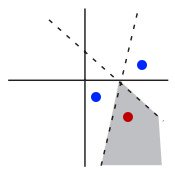
\includegraphics[width=175px, keepaspectratio]{3points.jpg}
\subsection*{B)}
The VC-dimension of this hypthesis class is 5. This is because it can
shatter all configurations of 4 points. However, it would not be able to do so for all
configuration of 5 points.
\subsection*{C)}
The VC-dimension of any type of boolean combination of 2 linear classifiers is
6. The reason is that we are not limited by conjunctions. This limitation is what
prevented us from shattering all configurations of 5 points in the previous example.
Now that this limitation is removed, we can succesfully shatter all combinations of 5
and we can atleast shatter one combination of 6 but not all. As such, the VC-dimension
in this case is 6.

\section*{Question 3}


$\left\{ (x_1,y_1),(x_2,y_2),...,(x_n,y_n)\right\}$.
Let $\delta[y=i]$ be 1 if $y=i$ and 0 otherwise. We write the likelihood function for a set of hypotheses and a given data set $D$ as follows:
$$L(h;D)=\prod_{i=1}^{n}\sum_{j=1}^{K}\delta[y_i=j]h^j(x_i)$$

\subsection*{A)}
Given the likelihood of an example x belonging to class k as being :

\begin{equation}
  L(k | x) = 1 - \sum_{i=1}^{K-1}h^i(x)
\end{equation}

In order to compute the likelihood of a set of hypotheses a composite likelihood
method can be used. This will approximate the likelihood of a set
of hypotheses given data set D:

\begin{equation}
  L(H | D) = \prod_{j=1}^K  L(h_j | d_j)
\end{equation}

Combining the likelihood of a given likelihood function with the composite method
we obtain the following likelihood function:

\begin{equation}
  L(H | D) = \prod_{j=1}^K
  \left(
  1 - \sum_{i=1}^{K-1}w_i^T x_i
  \right)
\end{equation}

This can be seen as the product of all the hypothesis likelihoods.

\subsection*{B)}
\begin{equation}
  \log L(H | D) = \log \sum_{j=1}^K
  \left(
  1 - \sum_{i=1}^{K-1}h_i(x_i)
  \right)
\end{equation}

\begin{equation}
  \log L(H | D) = \log
  \sum_{j=1}^K
  1 - \sum_{j=1}^K \sum_{i=1}^{K-1}h_i(x_i)
\end{equation}
The optimization is thus about minimizing:
\begin{equation}
  \sum_{j=1}^K \sum_{i=1}^{K-1}w_i^T x_i
\end{equation}
The loss function thus becomes:
\begin{equation}
  \log L(H | D) = \sum_{j=1}^K \sum_{i=1}^{K-1}w_i^T x_i
\end{equation}

\begin{equation}
  \frac{\partial}{\partial w} \log L(H | D) =
  \frac{\partial}{\partial w}
  \sum_{j=1}^K \sum_{i=1}^{K-1} x_i
\end{equation}


\subsection*{C)}

\newpage
\section*{Question 4}
\subsection*{A)}
\begin{center}
\begin{table}[h]
 \begin{tabular}{l|c|c|c|c|c|}
 \cline{2-6}
     & \multicolumn{5}{c|}{Folds}      \\ \cline{2-6}
     &  1  &  2  &  3  &  4  &  5 \\ \hline
\multicolumn{1}{|c|}{log L Train} & -0.410 & -0.408 & -0.409 & -0.433 & -0.422  \\ \hline
\multicolumn{1}{|c|}{log L Test} & -0.654 & -0.558 & -0.595 & -0.442 & -0.526  \\ \hline
\multicolumn{1}{|l|}{Training Accuracy} & 0.81\% & 0.81\% & 0.83\% & 0.81\% & 0.80\% \\ \hline
\multicolumn{1}{|l|}{Testing Accuracy} & 0.69\% & 0.69\% & 0.72\% & 0.87\% & 0.71\% \\ \hline
\end{tabular}
\end{table}
\end{center}


\subsection*{B)}
\begin{table}[h]
 \begin{tabular}{l|c|c|c|c|c|}
 \cline{2-6}
     & \multicolumn{5}{c|}{Folds}      \\ \cline{2-6}
     &  1  &  2  &  3  &  4  &  5 \\ \hline
\multicolumn{1}{|c|}{log L Train} & -0.049 & -0.067 & -0.026 & -0.028 & -0.183  \\ \hline
\multicolumn{1}{|c|}{log L Test} & -0.333 & -0.355 & -0.521 & -0.376 & -0.239  \\ \hline
\multicolumn{1}{|l|}{Training Accuracy} & 0.65\% & 0.65\% & 0.64\% & 0.65\% & 0.65\% \\ \hline
\multicolumn{1}{|l|}{Testing Accuracy} & 0.62\% & 0.62\% & 0.59\% & 0.54\% & 0.68\% \\ \hline
\end{tabular}
\end{table}


\subsection*{C)}
\begin{center}
\begin{table}[h]
 \begin{tabular}{l|c|c|c|c|c|}
 \cline{2-6}
     & \multicolumn{5}{c|}{Folds}      \\ \cline{2-6}
     &  1  &  2  &  3  &  4  &  5 \\ \hline
\multicolumn{1}{|c|}{log L Train} & -0.235 & -0.212 & -0.174 & -0.184 & -0.226  \\ \hline
\multicolumn{1}{|c|}{log L Test} & -0.530 & -0.611 & -0.803 & -0.633 & -0.536  \\ \hline
\multicolumn{1}{|l|}{Training Accuracy} & 0.83\% & 0.84\% & 0.83\% & 0.81\% & 0.83\% \\ \hline
\multicolumn{1}{|l|}{Testing Accuracy} & 0.72\% & 0.67\% & 0.69\% & 0.85\% & 0.74\% \\ \hline
\end{tabular}
\end{table}
\end{center}
\subsection*{D)}
Defining the sigmoid function as being:
\begin{equation}
  \sigma(a) = \frac{1}{1+e^{-a}}
\end{equation}
We can now express the standard logistic regression as:
\begin{equation}
  P(Y = 1 | X) = \sigma(w^TX + w_0) = \sigma(w_0 + \sum_{i=1}^{n}w_iX_i)
\end{equation}
\begin{equation}
  P(Y = 0 | X) = 1 - P(Y = 1 | X)
\end{equation}

Using a function $\phi$ mapping X from a low to a high dimension space we obtain
the following logistic regression:
\begin{equation}
  P(Y = 1 | \phi(X)) = \sigma(w_0 + \sum_{i=1}^{K}w_i\phi(X)_i)
\end{equation}
where K is the dimension of the new higher dimension space.\\
Using the kernel trick:
\begin{equation}
  P(Y = 1 | \phi(X)) = \sigma(\alpha_0 + \sum_{i=1}^{n}\alpha_iK(X_i,X))
\end{equation}
Combining equation 16, 17 and 19 we obtain the likelihood of $\alpha$

\begin{equation}
  \log L(\alpha) =
  \sum_{l=1}^{R} Y^l
  (\alpha_0 + \sum_{j=1}^{R}\alpha_j(X_j,X))
  -
  \log(1+\exp(\alpha_0 + \sum_{j=1}^{R}\alpha_j(X_j,X)))
\end{equation}

\begin{equation}
  \frac{\partial}{\partial \alpha_i} l(\alpha) =
  \sum_{l=1}^{R}\left(Y^l -
  \frac{
  \exp(\alpha_0 + \sum_{j=1}^{R}\alpha_j(X_j,X))
  }{
  1+\exp(\alpha_0 + \sum_{j=1}^{R}\alpha_j(X_j,X))
  }
  \right)
  K(X_I,X)
\end{equation}

\begin{equation}
    \alpha_{t+1} = \alpha_t + \gamma K(y - \hat{y})
\end{equation}

\subsection*{E)}

\end{document}
